% vim:ft=tex
% rubber: module xelatex
\subsection{Image segmentation}
\label{sec:segmentation}

We implemented two image segmentation algorithms: a simple thresholding algorithm, and a split and merge algorithm as described in the lecture slides. Each algorithm takes as input a greyscale image and outputs a segmented image. In the simple thresholding case, the output image is divided into binary regions. In the case of the split and merge algorithm, the output image is divided into arbitrarily many regions, each assigned a greyscale colour from a rotating set of grey values.

\subsubsection{Implementation notes}

The `global threshold' form of the thresholding algorithm takes the mean of all the pixel intensities in the image, and sorts each pixel as belonging to the background or the foreground based on this threshold. The `adaptive threshold' option begins with the global threshold, then iteratively adjusts it to be halfway between the means of the current background and foreground, adjusting what qualifies as a background or foreground pixel accordingly until the threshold converges. This simple algorithm has a user parameter which sets whether the background in the original image is light or dark.

The split and merge algorithm is a form of contextual segmentation. The image begins as a single region. In each iteration of the ``split" step, every region is quartered into subregions. This process continues until all regions are uniform according to the uniformity predicate based on the value $\Delta$. Then the ``merge" step begins. In each iteration, adjacent regions are merged if the uniformity predicate would hold for the resulting superregion. Typically, the behaviour of the ``split" step would require that the input image has width and height that are powers of 2. This restriction is overcome by padding the edges with zero-intensity pixels to extend the image to the nearest power of 2. Regions made entirely of zero-padding are then removed before the "merge" step. Regions made partly of zero-padding are included in the "merge" step, but the resulting image is cropped back to its original parameters for the display.

In our implementation, the split and merge algorithm represents regions using the Region class. Unfortunately, in an attempt to be more efficient (by storing and processing fewer pixels), the Region class only stores the points of the regions' borders. The unforeseen downside of this is that the algorithm breaks down when there are non-convex regions: certain pixels are wrongly included in checks, causing some regions that should have been merged to escape the merging process. The result is that the segmentation process is less than perfect. The obvious solution to this implementation problem is to store all pixels which make up the region.

In the "merge" step of the split and merge segmentation, regions are compared to each other rather naively (i.e. every region is compared to every other region). This slows the implementation considerably when there are more than a few hundred regions after the split step (which occurs for low values of the delta parameter $\Delta$ and for extremely heterogeneous images). The solution would be to only consider merging regions that are neighbouring; this is unfortunately impossible to do efficiently with our current region representation. Regions are merged using 4-connectivity, in as far as the algorithm checks, for each pixel on the boundary of a region, in four directions to determine whether the region can be merged.

\subsubsection{Experimental process}

\paragraph{Subjective rating.}
We performed a small qualitative test of the usefulness of the thresholding algorithms and the split and merge algorithm. In this test, we took randomly generated words as the basis for 20 Google searches, and ran the segmenting algorithms on the third image returned in each case. We rated the output of the adaptive thresholding algorithm as `better' in 13 cases, and of these, the adaptive threshold was significantly different (20+ units difference) from the global threshold in 10 cases. For 4 of the images, the adaptive and global thresholds gave almost identical results; in each of these cases, the global threshold was within 20 units of the adaptive threshold. We rated the global threshold as `better' than the adaptive threshold in just 3 cases. These were comprised of:
\begin{itemize}
   \item \emph{A complex image of a brightly-lit bridge.} The global threshold picked out some of the detail of the spars that the adaptive threshold did not.
   \item \emph{An image of a cartoon character.} The global threshold picked out important text in an intensity similar to the background of that text. The adaptive threshold failed to pick out this text.
   \item \emph{An image of a boat in the Waitomo caves.} The global threshold was better able to pick out the glow-worms and the bow of the boat.
\end{itemize}
In all cases, the split and merge algorithm performed poorly due to the issues we have mentioned. For the thresholding algorithm, there appeared (subjectively) to be a correlation between the quality of the segmentation and the difference between the global and adaptive threshold, in that the adaptive threshold \emph{usually} appeared to perform better when this difference was significant.

\paragraph{Region-counting experiment.}
For a basic test of the split and merge algorithm's capabilities, we took four small test images from our photos of the camera calibration object (see section~\ref{sec:calibration}): one image with two regions, one with five regions, one with seven regions and one with ten regions. For each test image, we ran the split and merge algorithm with varying $\Delta$ values.

The results are presented in figure~\ref{fig:region-counts}. As expected, the higher the value $\Delta$, the fewer regions are returned (a more relaxed uniformity predicate allows more regions to be merged). We observe that an appropriate value of $\Delta$ for an image of relatively few regions appears to be between 100 and 150. We should note, however, that the current implementation of the algorithm fails on non-convex regions, and the 'best' $\Delta$ value may be different for a better implementation. Note also that returning the \emph{correct number} of regions is not the same as accurately determining \emph{what} those regions should be.

\begin{figure}[h]
  \centering
  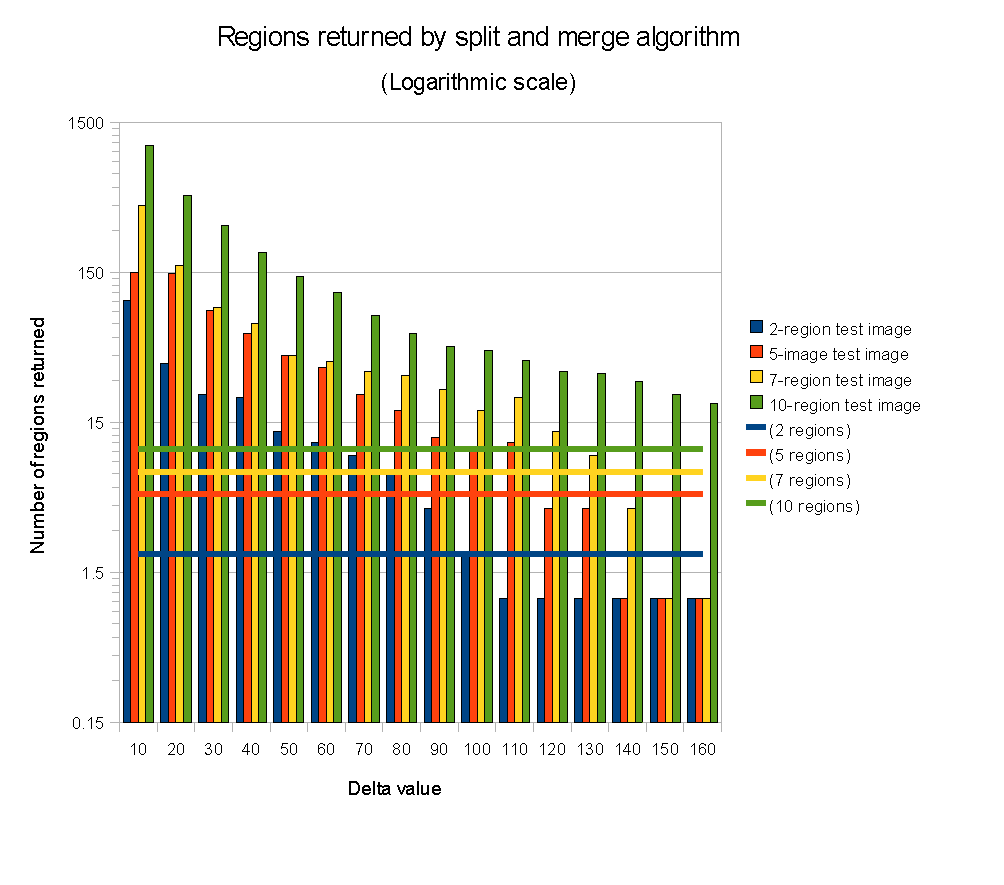
\includegraphics[width=0.8\textwidth]{figures/region-counts}
  \caption[Regions returned by split and merge algorithm]{Number of regions returned by the split and merge algorithm. The graph shows the region count for four test images. A horizontal line of the appropriate colour shows the manually-determined correct number of regions for each image.}
  \label{fig:region-counts}
\end{figure}
